\documentclass[12pt, titlepage]{article}

\usepackage[section]{placeins}
\usepackage{makecell}
\usepackage{booktabs}
\usepackage{tabularx}
\usepackage{hyperref}
\usepackage{attachfile}
\usepackage{graphicx}
\hypersetup{
    colorlinks,
    citecolor=black,
    filecolor=black,
    linkcolor=red,
    urlcolor=blue
}
\usepackage[round]{natbib}

\title{SE 3XA3: Test Report\\TankWar}

\author{Team \#212, Genius
		\\Di Wu, 400117248, wud43 
		\\Jiahao Zhou, 400082351, zhouj56 
		\\Xinyu Huang, 400120376, huangx65
}

\date{\today}



\begin{document}

\maketitle

\pagenumbering{roman}
\tableofcontents
\listoftables
\listoffigures

\begin{table}[bp]
\caption{\bf Revision History}
\begin{tabularx}{\textwidth}{p{3cm}p{2cm}X}
\toprule {\bf Date} & {\bf Version} & {\bf Notes}\\
\midrule
27 March 2020 & 1.0 & Create the first version of the Test Plan\\
 2020 & 1.1 & Finish all the parts of the Test Report\\
\bottomrule
\end{tabularx}
\end{table}

\newpage

\pagenumbering{arabic}

This document provides a report that describes the results of the testing for the TankWar game. The test result of functional and nonfunctional requirements, and unit testing are presented in the file. The traceability of this test report to requirements and modules are showed.
Note that all test cases conducted in this report are described in the Test Plan document. Please refer to the Test Plan for the details.

\section{Functional Requirements Evaluation}

\subsection{Area of Testing1 for Tank Movements}
There are four sections in Tank Movements: going up, going down, going left, and going right. The test cases of each sections are similar. Here is the test results for going up section.
\paragraph{Test for Going Up}

\begin{enumerate}

\item{MT-GU-1\\}
					
Initial State: After the game starts.
					
Input: "W" key held by player 1.
					
Expected result: Player 1's tank goes up, which is shown on the screen.
					
Actual result: The screen shows the action that player 1's tank going up.

Result: pass
					
\item{MT-GU-2\\}
					
Initial State: After the game starts.
					
Input: "W" key pressed by player 1.
					
Expected result: Player 1's tank goes up by 1 unit of length, which is shown on the screen.
					
Actual result: Player 1's tank goes up by 1 unit of length. The screen shows the action simultaneously.

Result: pass

\item{MT-GU-3\\}
					
Initial State: After the double-life tank is shot by a bullet and the ultimate skill is activated.
					
Input: "W" key held by player 1.
					
Expected result: Player 1's double-life tank still goes up, which is shown on the screen.
					
Actual result: Player 1's double-life tank still goes up. The screen shows the action simultaneously.

Result: pass

\item{MT-GU-4\\}
					
Initial State: After the double-life tank is shot by a bullet and the ultimate skill is activated.
					
Input: "W" key pressed by player 1.
					
Expected result: Player 1's double-life tank still goes up by 1 unit of length, which is shown on the screen.
					
Actual result: Player 1's double-life tank still goes up by 1 unit of length. The screen shows the action simultaneously.

Result: pass

\item{MT-GU-5\\}
					
Initial State: After the game starts.
					
Input: Upward Arrow key held by player 2.
					
Expected result: Player 2's tank goes up, which is shown on the screen.
					
Actual result: Player 2's tank goes up. The screen shows the action simultaneously. 
			
Result: pass

\item{MT-GU-6\\}
					
Initial State: After the game starts.
					
Input: Upward arrow key pressed by player 2.
					
Expected result: Player 2's tank goes up by 1 unit of length, which is shown on the screen.
					
Actual result: Player 1's tank goes up by 1 unit of length. The screen shows the action simultaneously.

Result: pass

\item{MT-GU-7\\}
					
Initial State: After the double-life tank is shot by a bullet and the ultimate skill is activated.
					
Input: Upward arrow key held by player 2.
					
Expected result: Player 2's double-life tank still goes up, which is shown on the screen.
					
Actual result: Player 2's double-life tank still goes up. The screen shows the action simultaneously.

Result: pass

\item{MT-GU-8\\}
					
Initial State: After the double-life tank is shot by a bullet and the ultimate skill is activated.
					
Input: Upward arrow key pressed by player 2.
					
Expected result: Player 2's double-life tank still goes up by 1 unit of length, which is shown on the screen.
					
Actual result: Player 2's double-life tank still goes up by 1 unit of length. The screen shows the action simultaneously.

Result: pass

\end{enumerate}

The rest of the test cases are also completed and get the expected results. The techniques of testing the rest three sections are similar to the Going Up section above, which is to test player 1's operation keys and player 2's operation keys separately. Also the moving ability of double-life tank is tested after getting shot by one bullet. 

\paragraph{Test for Walls and Boundaries}

\begin{enumerate}

\item{MT-WB-1\\}
					
Initial State: After the game starts.
					
Input: Player 1's tank is facing to a brick wall and there is no distance between the tank and the wall. Player 1 presses the corresponding key from "WASD" keys in order to make the tank move towards the brick wall.
					
Expected result: Player 1's tank does not move.
					
Actual result: Player 1's tank stops.

Result: pass

\item{MT-WB-2\\}
					
Initial State: After the game starts.
					
Input: Player 1's tank is facing to a iron wall and there is no distance between the tank and the wall. Player 1 presses the corresponding key from "WASD" keys in order to make the tank move towards the iron wall.
					
Expected result: Player 1's tank does not move.
					
Actual result: Player 1's tank stops.

Result: pass

\item{MT-WB-3\\}
					
Initial State: After the game starts.
					
Input: Player 2's tank is facing to a brick wall and there is no distance between the tank and the wall. Player 2 presses the corresponding key from arrow keys in order to make the tank move towards the brick wall.
					
Expected result: Player 2's tank does not move.
					
Actual result: Player 2's tank stops.

Result: pass

\item{MT-WB-4\\}
					
Initial State: After the game starts.
					
Input: Player 2's tank is facing to a iron wall and there is no distance between the tank and the wall. Player 2 presses the corresponding key from arrow keys in order to make the tank move towards the iron wall.
					
Expected result: Player 2's tank does not move.
					
Actual result: Player 2's tank stops.

Result: pass

\item{MT-WB-5\\}
					
Initial State: After the game starts.
					
Input: Player 2's tank is facing to the boundary of the map and there is no distance between the tank and the boundary. Player 2 presses the corresponding key from arrow keys in order to make the tank move towards the boundary.
					
Expected result: Player 2's tank does not move.
					
Actual result: Player 2's tank stops.

Result: pass

\item{MT-WB-6\\}
					
Initial State: After the game starts.
					
Input: Player 1's tank is facing to the boundary of the map and there is no distance between the tank and the boundary. Player 1 presses the corresponding key from "WASD" keys in order to make the tank move towards the boundary.
					
Expected result: Player 1's tank does not move.
					
Actual result: Player 1's tank stops.

Result: pass

\end{enumerate}

\subsection{Area of Testing2 for Tank Attacking}

\paragraph{Test for Shooting Bullets}

\begin{enumerate}

\item{TAT-SB-1\\}
					
Initial State: After the game starts.
					
Input: "J" key pressed by player 1.
					
Expected result: Player 1's tank shoots a bullet.
					
Actual result: Player 1's tank shoots a bullet.

Result: pass

\item{TAT-SB-2\\}
					
Initial State: After the game starts.
					
Input: "J" key held by player 1.
					
Expected result: Player 1's tank shoots bullets continuously. 
					
Actual result: Player 1's tank shoots bullets continuously. 

Result: pass

\item{TAT-SB-3\\}
					
Initial State: After the game starts.
					
Input: "," key pressed by player 2.
					
Expected result: Player 2's tank shoots a bullet.
					
Actual result: Player 2's tank shoots a bullet.

Result: pass

\item{TAT-SB-4\\}
					
Initial State: After the game starts.
					
Input: "," key held by player 2.
					
Expected result: Player 2's tank shoots bullets continuously. 
					
Actual result: Player 2's tank shoots bullets continuously.

Result: pass

\item{TAT-SB-5\\}
					
Initial State: After the double-life tank get shot for the first time.
					
Input: "," key held by player 2.
					
Expected result: Player 2's double-life tank still shoots bullets continuously.
					
Actual result: Player 2's double-life tank still shoots bullets continuously.

Result: pass

\item{TAT-SB-6\\}
					
Initial State: After the double-life tank get shot for the first time.
					
Input: "J" key held by player 1.
					
Expected result: Player 1's double-life tank still shoots bullets continuously.
					
Actual result: Player 1's double-life tank still shoots bullets continuously.

Result: pass

\item{TAT-SB-7\\}
					
Initial State: After the double-life tank get shot for the first time.
					
Input: "," key pressed by player 2.
					
Expected result: Player 2's double-life tank still shoots a bullet.
					
Actual result: Player 2's double-life tank still shoots a bullet.

Result: pass

\item{TAT-SB-8\\}
					
Initial State: After the double-life tank get shot for the first time.
					
Input: "J" key pressed by player 1.
					
Expected result: Player 1's double-life tank still shoots a bullet.
					
Actual result: Player 1's double-life tank still shoots a bullet.

Result: pass

\end{enumerate}

\paragraph{Test for Using Ultimate Skills}

\begin{enumerate}

\item{TAT-UUS-1\\}
					
Initial State: After the game starts.
					
Input: "K" key pressed by player 1.
					
Expected result: Player 1's tank use ultimate skills.
					
Actual result: Player 1's tank use ultimate skills.

Result: pass

\item{TAT-UUS-2\\}
					
Initial State: After the game starts.
					
Input: "." key pressed by player 2.
					
Expected result: Player 2's tank use ultimate skills.
					
Actual result: Player 2's tank use ultimate skills.

Result: pass

\item{TAT-UUS-3\\}
					
Initial State: After the game starts.
					
Input: "K" key held by player 1.
					
Expected result: Player 1's tank use ultimate skills continuously.
					
Actual result: Player 1's tank use ultimate skills continuously.

Result: pass

\item{TAT-UUS-4\\}
					
Initial State: After the game starts.
					
Input: "." key held by player 2.
					
Expected result: Player 2's tank use ultimate skills continuously.
					
Actual result: Player 2's tank use ultimate skills continuously.

Result: pass

\end{enumerate}

\subsection{Area of Testing3 for Tank Properties}

\paragraph{Test for Double-Life Tank}

\begin{enumerate}

\item{TPT-DLT-1\\}
					
Initial State: After the game starts.
					
Input: Player chooses double-life tank before entering the game and the player presses "K" key or "." key to activate the ultimate skill.
					
Expected result: The double-life tank is still alive when the ultimate skill is activated and the tank gets shot simultaneously.
					
Actual result: The double-life tank is still alive.

Result: pass

\end{enumerate}

\paragraph{Test for High-Speed Tank}

\begin{enumerate}

\item{TPT-HST-1\\}
					
Initial State: After the game starts.
					
Input: Player chooses high-speed tank before entering the game and the player presses "K" key or "." key to activate the ultimate skill.
					
Expected result: During the tank movement, the tank rushes for 1 seconds after the ultimate skill is activated. The direction can be changed by the player during the rushing process by pressing another key on the keyboard.
					
Actual result: The ultimate skill only available for 1 second. During the time, the speed of tank becomes faster and direction can be changed during rushing time. After 1 second, the speed of tank returns normal.

Result: pass

\end{enumerate}

\paragraph{Test for Double-Bullet Tank}

\begin{enumerate}

\item{TPT-DBT-1\\}
					
Initial State: After the game starts.
					
Input: Player chooses double-bullet tank before entering the game and the player presses "K" key or "." key on the keyboard to activate the ultimate skill.
					
Expected result: During attacking, the double-bullet tank shoots two bullets simultaneously when the ultimate skill activates. 
					
Actual result: The double-bullet tank shoots two bullets simultaneously, one with a faster speed and another with a slower speed.

Result: pass

\end{enumerate}

\subsection{Area of Testing4 for Gaming Process}

\paragraph{Test for \underline{PVP} Mode Selection}

\begin{enumerate}

\item{GPT-PPMS-1\\}
					
Initial State: Player 1 opens the software.
					
Input: Player 1 selects \underline{PVP} mode using ENTER key as the button of confirming from the keyboard.
					
Expected result: After opening the software, there should be three modes for player to choose. If the player chooses \underline{PVP} mode, there should be the interface for \underline{PVP} tank selection shown on the screen. 
					
Actual result: After pressing the Enter key, the interface of tank selection is shown.

Result: pass

\end{enumerate}

\paragraph{Test for \underline{PVE} Mode Selection}

\begin{enumerate}

\item{GPT-PEMS-1\\}
					
Initial State: Player 1 opens the software.
					
Input: Player 1 selects \underline{PVE} mode using Enter key as the button of confirming from the keyboard.
					
Expected result: After opening the software, there should be three modes for player to choose. If the player chooses \underline{PVE} mode, there should be the interface for \underline{PVE} tank selection shown on the screen. 
					
Actual result: After pressing the Enter key, the interface of tank selection is shown.

Result: pass

\end{enumerate}

\paragraph{Test for Map Editing Mode Selection}

\begin{enumerate}

\item{GPT-MEMS-1\\}
					
Initial State: Player 1 opens the software.
					
Input: Player 1 selects map editing mode using Enter key as the button of confirming from the keyboard.
					
Expected result: After opening the software, there should be three modes for player 1 to choose. If the player 1 chooses map editing mode, there should be the interface for map selection shown on the screen.
					
Actual result: After pressing the Enter key, the interface of choosing map is shown.

Result: pass

\end{enumerate}

\paragraph{Test for \underline{PVP} Map Loading}

\begin{enumerate}

\item{GPT-PPML-1\\}
					
Initial State: Player 1 opens the software and selects \underline{PVP} mode using Enter key as the button of confirming from the keyboard.
					
Input: Player 1 selects one of the \underline{PVP} maps in the \underline{PVP} map selecting section.
					
Expected result: The selected \underline{PVP} map shows on the screen.
					
Actual result: The selected \underline{PVP} map shows on the screen.

Result: pass

\end{enumerate}

\paragraph{Test for \underline{PVE} Map Loading}

\begin{enumerate}

\item{GPT-PEML-1\\}
					
Initial State: Player 1 opens the software and selects \underline{PVE} mode using Enter key as the button of confirming from the keyboard.
					
Input: Player 1 selects one of the \underline{PVE} maps in the \underline{PVE} map selecting section.
					
Expected result: The selected \underline{PVE} map shows on the screen.
					
Actual result: The selected \underline{PVE} map shows on the screen.

Result: pass

\end{enumerate}

\paragraph{Test for \underline{PVP} Tank Selection}

\begin{enumerate}

\item{GPT-PPTS-1\\}
					
Initial State: Player 1 opens the software, selects \underline{PVP} mode by using Enter key as the button of confirming from the keyboard.
					
Input: Player 1 chooses one from three different kinds of tanks by using Enter key as the button of confirming from the keyboard.
					
Expected result: The corresponding tank shows on the selected \underline{PVP} map.
					
Actual result: The corresponding tank shows on the selected \underline{PVP} map.

Result: pass

\item{GPT-PPTS-2\\}
					
Initial State: Player 1 opens the software, selects \underline{PVP} mode by using Enter key as the button of confirming from the keyboard.
					
Input: Player 2 chooses one from three different kinds of tanks using Enter key as the button of confirming from the keyboard.
					
Expected result: The corresponding tank shows on the selected \underline{PVP} map.
					
Actual result: The corresponding tank shows on the selected \underline{PVP} map.

Result: pass

\end{enumerate}

\paragraph{Test for \underline{PVE} Tank Selection}

\begin{enumerate}

\item{GPT-PETS-1\\}
					
Initial State: Player 1 opens the software, selects \underline{PVE} mode by using Enter key as the button of confirming from the keyboard.
					
Input: Player 1 chooses one from three different kinds of tanks by using Enter key as the button of confirming from the keyboard.
					
Expected result: The corresponding tank shows on the selected \underline{PVE} map.
					
Actual result: The corresponding tank shows on the selected \underline{PVE} map.

Result: pass

\item{GPT-PETS-2\\}
					
Initial State: Player 1 opens the software, selects \underline{PVE} mode by using Enter key as the button of confirming from the keyboard.
					
Input: Player 2 chooses one from three different kinds of tanks using Enter key as the button of confirming from the keyboard.
					
Expected result: The corresponding tank shows on the selected \underline{PVE} map.
					
Actual result: The corresponding tank shows on the selected \underline{PVE} map.

Result: pass

\end{enumerate}




\subsection{Area of Testing5 for Map Editing}

\paragraph{Test for Adding Brick Wall for \underline{PVP} Map}

\begin{enumerate}

\item{ME-\underline{PVP}AB-1\\}
					
Initial State: The map editing for \underline{PVP} mode is running, and there is empty space in front of the player's tank.
					
Input: "J" key pressed.
					
Expected result: A brick wall is added right in front of the player's tank.
					
Actual result: A brick wall is added right in front of the player's tank.
					
Result: pass

\item{ME-\underline{PVP}AB-2\\}
					
Initial State: The map editing for \underline{PVP} mode is running, and the player's tank is facing to a brick wall.
					
Input: "J" key pressed.
					
Expected result: Nothing is changed.
					
Actual result: The map editing for \underline{PVP} mode will be run and the player's tank will be moved to face to and with no distance with a existing brick wall, then the "K" key will be pressed and check if nothing is changed.

Result: pass

\item{ME-PVPAB-3\\}
					
Initial State: The map editing for \underline{PVP} mode is running, and the player's tank is facing to a iron wall.
					
Input: "J" key pressed.
					
Expected result: Nothing is changed.
					
Actual result: Nothing is changed.

Result: pass

\item{ME-PVPAB-4\\}
					
Initial State: The map editing for \underline{PVP} mode is running, and the player's tank is facing the boundary of the map.
					
Input: "J" key pressed.
					
Expected result: Nothing is changed.
					
Actual result: Nothing is changed.

Result: pass

\end{enumerate}


\paragraph{Test for Adding Iron Wall for \underline{PVP} Map}

\begin{enumerate}

\item{ME-PVPAI-1\\}
					
Initial State: The map editing for \underline{PVP} mode is running, and there is empty space in front of the player's tank.
					
Input: "K" key pressed.
					
Expected result: A iron wall is added right in front of the player's tank.
					
Actual result: A iron wall is added right in front of the player's tank.

Result: pass

\item{ME-PVPAI-2\\}
					
Initial State: The map editing for \underline{PVP} mode is running, and the player's tank is facing to a brick wall.
					
Input: "K" key pressed.
					
Expected result: Nothing is changed.
					
Actual result: Nothing is changed.

Result: pass

\item{ME-PVPAI-3\\}
					
Initial State: The map editing for \underline{PVP} mode is running, and the player's tank is facing to a iron wall.
					
Input: "K" key pressed.
					
Expected result: Nothing is changed.
					
Actual result: Nothing is changed.

Result: pass

\item{ME-PVPAI-4\\}
					
Initial State: The map editing for \underline{PVP} mode is running, and the player's tank is facing to the boundary of the map.
					
Input: "K" key pressed
					
Expected result: Nothing is changed.
					
Actual result: Nothing is changed.

Result: pass

\end{enumerate}


\paragraph{Test for Deleting Wall for \underline{PVP} Map}

\begin{enumerate}

\item{ME-PVPDW-1\\}
					
Initial State: The map editing for \underline{PVP} mode is running, and the player's tank is aim at a brick wall.
					
Input: "L" key pressed
					
Expected result: The brick wall is deleted from the map.
					
Actual result: The brick wall is deleted from the map.

Result: pass

\item{ME-PVPDW-2\\}
					
Initial State: The map editing for \underline{PVP} mode is running, and the player's tank is aim at a iron wall.
					
Input: "L" key pressed
					
Expected result: The iron wall is deleted from the map.
					
Actual result: The iron wall is deleted from the map.

Result: pass

\item{ME-PVPDW-3\\}
					
Initial State: The map editing for \underline{PVP} mode is running, and the player's tank is aim at nothing.
					
Input: "L" key pressed
					
Expected result: Nothing is changed in the map.
					
Actual result: Nothing is changed in the map.

Result: pass

\end{enumerate}

\paragraph{Test for Adding Brick Wall for \underline{PVE} Map\\}

For PVE map, the testing strategy is same as PVP map. Firstly, the ability of adding brick should be tested, including the situations about adding the brick on a free space, adding the brick on the area with another brick or iron, and adding the brick on the boundary of map. Secondly, the ability of adding iron should be tested, including the situations about adding the iron on a free space, adding the iron on the area with another brick or iron, and adding the iron on the boundary of map. Lastly, deleting ability should be tested, including deleting a brick wall, deleting a iron wall, and pressing "L" facing a free space. The results for those test cases in PVE map are same as expected.

\paragraph{Test for Saving Maps for \underline{PVP}}

\begin{enumerate}

\item{ME-PVPSM-1\\}
					
Initial State: The player is in map editing mode and a map is created.
					
Input: Press the "Enter" key, then enter a valid file name and press "Enter" key again.
					
Expected result: A file stands for the map created is shown in the folder for \underline{PVP} maps.
					
Actual result: A file stands for the map created is shown in the folder for \underline{PVP} maps.

Result: pass

\end{enumerate}

\paragraph{Test for Saving Maps for \underline{PVE}}

\begin{enumerate}

\item{ME-\underline{PVE}SM-1\\}
					
Initial State: The player is in map editing mode and a map is created.
					
Input: Press the "Enter" key, then select the existing files and press "Enter" key again.
					
Expected result: A file stands for the map created is shown in the folder for \underline{PVE} maps.
					
Actual result: A file stands for the map created is shown in the folder for \underline{PVE} maps.

Result: pass

\end{enumerate}

\subsection{Area of Testing6 for Game Rules}

\paragraph{Test for General Rules about the Wall}

\begin{enumerate}

\item{GR-GRW-1\\}
					
Initial State: After the \underline{PVP} game starts. 
					
Input: Player 1 presses "J" key from the keyboard to shoot a bullet towards the brick wall and the bullet hits the brick wall.
					
Expected result: The brick wall is destroyed by the bullet. The bullet and the brick wall disappear simultaneously.
					
Actual result: The brick wall is destroyed by the bullet. The bullet and the brick wall disappear simultaneously.

Result: pass

\item{GR-GRW-2\\}
					
Initial State: After the \underline{PVE} game starts. 
					
Input: Player 1 presses "J" key from the keyboard to shoot a bullet towards the brick wall and the bullet hits the brick wall.
					
Expected result: The brick wall is destroyed by the bullet. The bullet and the brick wall disappear simultaneously.
					
Actual result: The brick wall is destroyed by the bullet. The bullet and the brick wall disappear simultaneously.

Result: pass

\item{GR-GRW-3\\}
					
Initial State: After the \underline{PVE} game starts. 
					
Input: Player 2 presses "," key from the keyboard to shoot a bullet towards the brick wall and the bullet hits the brick wall.
					
Expected result: The brick wall is destroyed by the bullet. The bullet and the brick wall disappear simultaneously.
					
Actual result: The brick wall is destroyed by the bullet. The bullet and the brick wall disappear simultaneously.

Result: pass

\item{GR-GRW-4\\}
					
Initial State: After the \underline{PVP} game starts. 
					
Input: Player 2 presses "," key from the keyboard to shoot a bullet towards the brick wall and the bullet hits the brick wall.
					
Expected result: The brick wall is destroyed by the bullet. The bullet and the brick wall disappear simultaneously.
					
Actual result: The brick wall is destroyed by the bullet. The bullet and the brick wall disappear simultaneously.

Result: pass




\item{GR-GRW-5\\}
					
Initial State: After the \underline{PVP} game starts. 
					
Input: Player 1 presses "J" key from the keyboard to shoot a bullet towards the iron wall and the bullet hits the iron wall.
					
Expected result: The iron wall is not destroyed by the bullet. The bullet disappear.
					
Actual result: The iron wall is not destroyed by the bullet. The bullet disappear.

Result: pass

\item{GR-GRW-6\\}
					
Initial State: After the \underline{PVE} game starts. 
					
Input: Player 1 presses "J" key from the keyboard to shoot a bullet towards the iron wall and the bullet hits the iron wall.
					
Expected result: The iron wall is not destroyed by the bullet. The bullet disappear.
					
Actual result: The iron wall is not destroyed by the bullet. The bullet disappear.

Result: pass

\item{GR-GRW-7\\}
					
Initial State: After the \underline{PVE} game starts. 
					
Input: Player 2 presses "," key from the keyboard to shoot a bullet towards the iron wall and the bullet hits the iron wall.
					
Expected result: The iron wall is not destroyed by the bullet. The bullet disappear.
					
Actual result: The iron wall is not destroyed by the bullet. The bullet disappear.

Result: pass

\item{GR-GRW-8\\}
					
Initial State: After the \underline{PVP} game starts. 
					
Input: Player 2 presses "," key from the keyboard to shoot a bullet towards the iron wall and the bullet hits the iron wall.
					
Expected result: The iron wall is not destroyed by the bullet. The bullet disappear.
					
Actual result: The iron wall is not destroyed by the bullet. The bullet disappear.

Result: pass

\end{enumerate}

\paragraph{Test for General Rules about Buff}

\begin{enumerate}

\item{GR-GRB-2\\}
					
Initial State: After the \underline{PVE} game starts. 
					
Input: Two players enter the \underline{PVE} game successfully.
					
Expected result: Different buffs randomly appear in the different locations of the map during a random time period.
					
Actual result: Different buffs randomly appear in the different locations of the map during a random time period.

Result: pass

\item{GR-GRB-6\\}
					
Initial State: After the \underline{PVE} game starts. 
					
Input: The player gets the moving-speed-enhanced buff during the battle.
					
Expected result: The player's tank gets a higher speed after getting the moving-speed-enhanced buff. The moving-speed-enhanced buff disappear after the player's tank gets it.
					
Actual result: The player's tank gets a higher speed after getting the moving-speed-enhanced buff. The moving-speed-enhanced buff disappear after the player's tank gets it.

Result: pass

\item{GR-GRB-7\\}
					
Initial State: After the \underline{PVE} game starts. 
					
Input: The player gets the wall-enhanced buff during the battle.
					
Expected result: The player's home base is surrounded by iron walls instead of brick walls. The wall-enhanced buff disappears after the player's tank gets it.
					
Actual result: The player's home base is surrounded by iron walls instead of brick walls. The wall-enhanced buff disappears after the player's tank gets it.

Result: pass

\item{GR-GRB-8\\}
					
Initial State: After the \underline{PVE} game starts. 
					
Input: The player gets the bullet-speed-enhanced buff during the battle.
					
Expected result: Bullets shot by the player's tank gets a higher moving speed. The bullet-speed-enhanced buff disappears after the player's tank gets it.
					
Actual result: Bullets shot by the player's tank gets a higher moving speed. The bullet-speed-enhanced buff disappears after the player's tank gets it.

Result: pass

\end{enumerate}

\paragraph{Test for General Rules about Lifes}

\begin{enumerate}

\item{GR-GRL-1\\}
					
Initial State: After the \underline{PVP} game starts. 
					
Input: Player 1 controls the tank using "WASD" keys from the keyboard and drives the tank towards the bullet shot by the player 2's tank for three times. The bullet hits player 1's tank three times.
					
Expected result: Player 1's tank relives for the first and second time after hit by the bullet shot by player 2's tank. Player 1's tank does not relive after the third-time hit by the bullet.
					
Actual result: Player 1's tank relives for the first and second time after hit by the bullet shot by player 2's tank. Player 1's tank does not relive after the third-time hit by the bullet.

Result: pass

\item{GR-GRL-2\\}
					
Initial State: After the \underline{PVP} game starts.
					
Input: Player 2 controls the tank using "WASD" keys from the keyboard and drives the tank towards the bullet shot by the player 1's tank for three times. The bullet hits player 2's tank three times.
					
Expected result: Player 2's tank relives for the first and second time after hit by the bullet shot by player 1's tank. Player 2's tank does not relive after the third-time hit by the bullet.
					
Actual result: Player 2's tank relives for the first and second time after hit by the bullet shot by player 1's tank. Player 2's tank does not relive after the third-time hit by the bullet.

Result: pass

\item{GR-GRL-3\\}
					
Initial State: After the \underline{PVE} game starts.
					
Input: Player 1 controls the tank using "WASD" keys from the keyboard and drives the tank towards the bullet shot by the enemy tanks for three times. The bullet hits player 1's tank three times.
					
Expected result: Player 1's tank relives for the first and second time after hit by the bullet shot by enemy tanks. Player 1's tank does not relive after the third-time hit by the bullet.
					
Actual result: Player 1's tank relives for the first and second time after hit by the bullet shot by enemy tanks. Player 1's tank does not relive after the third-time hit by the bullet.

Result: pass

\item{GR-GRL-4\\}
					
Initial State: After the \underline{PVE} game starts.
					
Input: Player 2 controls the tank using "WASD" keys from the keyboard and drives the tank towards the bullet shot by the enemy tanks for three times. The bullet hits player 2's tank three times.
					
Expected result: Player 2's tank relives for the first and second time after hit by the bullet shot by enemy tanks. Player 2's tank does not relive after the third-time hit by the bullet.
					
Actual result: Player 2's tank relives for the first and second time after hit by the bullet shot by enemy tanks. Player 2's tank does not relive after the third-time hit by the bullet.

Result: pass

\end{enumerate}

\paragraph{Test for General Rules about Timing}

\begin{enumerate}

\item{GR-GRT-1\\}
					
Initial State: After the \underline{PVP} game starts.
					
Input: Player 1 and player 2 enter the \underline{PVP} game successfully.
					
Expected result: Player 1 and player 2 participate a \underline{PVP} game for at most 3 minutes, if the two home bases are not destroyed and no player's tank is destroyed for 3 times.
					
Actual result: The game ends after 3 minutes.

Result: pass

\item{GR-GRT-2\\}
					
Initial State: After the \underline{PVE} game starts.
					
Input: Player 1 and player 2 enter the \underline{PVE} game successfully.
					
Expected result: Player 1 and player 2 participate a \underline{PVE} game for at most 3 minutes, if the home base is not destroyed and no player's tank is destroyed for 3 times.
					
Actual result: The game ends after 3 minutes.

Result: pass

\end{enumerate}

\paragraph{Test for \underline{PVP} Rules}

\begin{enumerate}

\item{GR-PPR-1\\}
					
Initial State: After the \underline{PVP} game starts.
					
Input: Player 1 and player 2 enter the \underline{PVP} game successfully.
					
Expected result: There are two home bases shown on the \underline{PVP} map located on the left and right hand side of the map.
					
Actual result: There are two home bases shown on the \underline{PVP} map located on the left and right hand side of the map.

Result: pass

\item{GR-PPR-2\\}
					
Initial State: After the \underline{PVP} game starts.
					
Input: Player 1 and player 2 play for 3 minutes. No tank is destroyed three times and no tank destroys the other player's home base during this time period.
					
Expected result: A "Tie" is shown on the screen as the result of the game.
					
Actual result: A "Tie" is shown on the screen as the result of the game.

Result: pass

\item{GR-PPR-3\\}
					
Initial State: After the \underline{PVP} game starts.
					
Input: Player 1's tank destroys player 2's tank three times during the 3-minute period.
					
Expected result: A "Player 1 Win" is shown on the screen as the result of the game.
					
Actual result: A "Player 1 Win" is shown on the screen as the result of the game.

Result: pass

\item{GR-PPR-4\\}
					
Initial State: After the \underline{PVP} game starts.
					
Input: Player 2's tank destroys player 1's tank three times during the 3-minute period.
					
Expected result: A "Player 2 Win" is shown on the screen as the result of the game.
					
Actual result: A "Player 2 Win" is shown on the screen as the result of the game.

Result: pass

\item{GR-PPR-5\\}
					
Initial State: After the \underline{PVP} game starts.
					
Input: Player 2's tank destroys player 1's home base during the 3-minute period.
					
Expected result: A "Player 2 Win" is shown on the screen as the result of the game.
					
Actual result: A "Player 2 Win" is shown on the screen as the result of the game.

Result: pass

\item{GR-PPR-6\\}
					
Initial State: After the \underline{PVP} game starts.
					
Input: Player 1's tank destroys player 2's home base during the 3-minute period.
					
Expected result: A "Player 1 Win" is shown on the screen as the result of the game.
					
Actual result: A "Player 1 Win" is shown on the screen as the result of the game.

Result: pass

\end{enumerate}

\paragraph{Test for \underline{PVE} Rules}

\begin{enumerate}

\item{GR-PER-1\\}
					
Initial State: After the \underline{PVE} game starts.
					
Input: Player 1 and player 2 enter the \underline{PVE} game successfully.
					
Expected result: There is one home base shown on the \underline{PVE} map located on the bottom of the \underline{PVE} map.
					
Actual result: There is one home base shown on the \underline{PVE} map located on the bottom of the \underline{PVE} map.

Result: pass

\item{GR-PER-2\\}
					
Initial State: After the \underline{PVE} game starts.
					
Input: Player 1 and player 2 enter the \underline{PVE} game successfully.
					
Expected result: There is 5 enemy tanks created on the \underline{PVE} map after the \underline{PVE} mode starts.
					
Actual result: There is 5 enemy tanks created on the \underline{PVE} map after the \underline{PVE} mode starts. 

Result: pass

\item{GR-PER-3\\}
					
Initial State: After the \underline{PVE} game starts.
					
Input: Player 1 and player 2 enter the \underline{PVE} game successfully.
					
Expected result: Enemy tanks move by themselves. 
					
Actual result: Enemy tanks move by themselves. 

Result: pass

\item{GR-PER-4\\}
					
Initial State: After the \underline{PVE} game starts.
					
Input: Player 1 shoots a bullet to the enemy tank using "J" key from the keyboard. The bullet hits the enemy tank.
					
Expected result: Enemy tanks is destroyed by the bullet.
					
Actual result: Enemy tanks is destroyed by the bullet.

Result: pass

\item{GR-PER-5\\}
					
Initial State: After the \underline{PVE} game starts.
					
Input: Player 2 shoots a bullet to the enemy tank using "," key from the keyboard. The bullet hits the enemy tank.
					
Expected result: Enemy tanks is destroyed by the bullet.
					
Actual result: Enemy tanks is destroyed by the bullet.

Result: pass

\item{GR-PER-6\\}
					
Initial State: After the \underline{PVE} game starts.
					
Input: Player 1 and player 2 enter the \underline{PVE} game successfully.
					
Expected result: Enemy tanks shoot bullets automatically. 
					
Actual result: Enemy tanks shoot bullets automatically. 

Result: pass

\item{GR-PER-7\\}
					
Initial State: After the \underline{PVE} game starts.
					
Input: A enemy tank is destroyed.
					
Expected result: Another enemy tank relives.
					
Actual result: Another enemy tank relives.

Result: pass

\item{GR-PER-8\\}
					
Initial State: After the \underline{PVE} game starts.
					
Input: Players' home base is destroyed by the bullet shot by an enemy tank during the 3-minute period.
					
Expected result: A ”Lose” is shown on the screen as the result of the game.
					
Actual result: A ”Lose” is shown on the screen as the result of the game.

Result: pass

\item{GR-PER-9\\}
					
Initial State: After the \underline{PVE} game starts.
					
Input: The enemy tanks destroys player 1's and player 2's tanks three times each by using bullets during the 3-minute period.
					
Expected result: A ”Lose” is shown on the screen as the result of the game.
					
Actual result: A ”Lose” is shown on the screen as the result of the game.

Result: pass

\item{GR-PER-10\\}
					
Initial State: The \underline{PVE} game starts.
					
Input: Player  1  and  player  2  participate  the  \underline{PVE}  game  for  3 minutes. During the game, the home base is not destroyed and no player’s tank is destroyed for 3 times.
					
Expected result: A ”Win” is shown on the screen as the result of the game.
					
Actual result: A ”Win” is shown on the screen as the result of the game.

Result: pass

\end{enumerate}

\section{Nonfunctional Requirements Evaluation}

\subsection{Look and Feel}
\subsubsection{Visual Appearance Testing}
Description of the visual appearance testing: The test cases were conducted by the three developers from the project as the software testers and a test group of people as the test users from the society with different backgrounds among the age of 12 to 50. The participants in the tests were monitored and instructed to strictly follow the specification of the test cases from the test plan to perform the requested tasks. After finished the requested tasks, each participant would fill a feedback form or write a feedback reflection about the visual appearance testing.

\begin{enumerate}

\item{Test Name: LF-VA-1 \& LF-VA-2\\}

Description: The two test cases are similar. They are just in different initial state with the two mode PVP and PVE. So the tests would conducted by open the PVE mode and PVP mode respectively to play the game.

Initial State: The game is at PVE mode. PVE map is loaded and the players have chose tanks. /The game is at PVP mode. PVP map is loaded and the players have chose tanks.

Input/Condition: Players start the PVE game. /Players start the PVP game.

Expected Output: The screen shows the game in a 2-D drawing style.

Result: Pass. \\The drawing style of Tank War is in 2-D. No appearance is violated the required drawing style in both modes.

\item{Test Name: LF-VA-3\\}

Initial State: The game is installed on the computer.

Input/Condition: The game is just launched.

Expected Output: The screen shows the background of the game system in black.

Result: Pass. \\The background of the game is in black.

\item{Test Name: LF-VA-4 \& LF-VA-5\\}

Description: The two test cases are similar. They are just in different initial state with the two mode PVP and PVE. So the tests would conducted by open the PVE mode and PVP mode respectively to play the game.

Initial State: The game is at PVE mode. PVE map is loaded and the players have chose tanks. /The game is at PVP mode. PVP map is loaded and the players have chose tanks.

Input/Condition: Players start the PVE game. /Players start the PVP game.

Expected Output: The screen shows the brick walls and iron walls in a grid map.

Result: Pass. \\The brick walls and iron walls are in a grid map in both modes.

\item{Test Name: LF-VA-6 \& LF-VA-7\\}

Description: The two test cases are similar. They are just in different initial state with the two mode PVP and PVE. So the tests would conducted by open the PVE mode and PVP mode respectively to play the game.

Initial State: The game is at PVE mode. PVE map is loaded and the players have chose tanks. /The game is at PVP mode. PVP map is loaded and the players have chose tanks.

Input/Condition: Players start the PVE game. /Players start the PVP game.

Expected Output: The screen shows brick walls in orange and iron walls consisted of 4 iron cube in sliver, while the screen displays a home which looks like a eagle.

Result: Pass. \\The brick walls is in orange and iron walls consisted of 4 iron cube in sliver. The home is displayed and it looks like a eagle in both modes.

\item{Test Name: LF-VA-8 \& LF-VA-9\\}

Description: The two test cases are similar. They are just in different initial state with the two mode PVP and PVE. So the tests would conducted by open the PVE mode and PVP mode respectively to play the game.

Initial State: The game is at PVE mode and the PVE map is loaded. /The game is at PVP mode. PVP map is loaded.

Input/Condition: The two players choose two different types of tanks among double-life tank, high-speed tank, double-bullet tank. Then the players start the PVE game. /The two players choose two different types of tanks among double-life tank, high-speed tank, double-bullet tank. Then the players start the PVP game.

Expected Output: The two different types of tanks show on the screen with different colours.

Result: Pass. \\The different types of tanks show in different colours in both modes.

\item{Test Name: LF-VA-10 \& LF-VA-11\\}

Description: The two test cases are similar. They are just in different initial state with the two mode PVP and PVE. So the tests would conducted by open the PVE mode and PVP mode respectively to play the game.

Initial State: The game is at PVE mode and the PVE map is loaded and the players have chose tanks. /The game is at PVP mode. PVP map is loaded and the players have chose tanks.

Input/Condition: The players start the PVE game. /Players start the PVP game.

Expected Output: The drawing style of TankWar game is very similar to the drawing style of the original game ”Battle City”.

Result: Pass. \\The survey result from the 50 test users shows that there are 92 percent of the test users would consider that the drawing style of Tankwar is more than 90 percent similar with Battle City in both modes.

\end{enumerate}

\subsection{Usability and Humanity}
\subsubsection{Ease of Use Testing}
Description of the ease of use testing: The test cases were conducted by the three developers from the project as the software testers. The participants in the tests were monitored and instructed to strictly follow the specification of the test cases from the test plan to perform the requested tasks. After finished the requested tasks, each participant would fill a feedback form or write a feedback reflection about the ease of use testing.

\begin{enumerate}

\item{Test Name: UH-EU-1 \& UH-EU-2\\}

Description: The two test cases are similar. They are just in different initial state with the two mode PVP and PVE. So the tests would conducted by open the PVE mode and PVP mode respectively to play the game.

Initial State: The game is at PVE mode. PVE map is loaded. /The game is at PVP mode. PVP map is loaded.

Input/Condition: The players start to choose tanks.

Expected Output: The screen displays the photos and descriptions of different types of tanks to give a brief introduction when users are choosing tanks.

Result: Pass. \\There are instructions about each type of tanks in both modes.

\item{Test Name: UH-EU-3 \& UH-EU-4\\}

Description: The two test cases are similar. They are just in different initial state with the two mode PVP and PVE. So the tests would conducted by open the PVE mode and PVP mode respectively to play the game.

Initial State: The game is at PVE mode. PVE map is loaded and the players have chose tanks. /The game is at PVP mode. PVP map is loaded and the players have chose tanks.

Input/Condition: The players press ”Enter” key to start the PVE game. /The players press ”Enter” key to start the PVP game.

Expected Output: The rules of the game are displayed on the screen. If the players press the key "Enter", the game will start.

Result: Pass. \\The rules of the game are displayed on the screen in both modes. Once the players press the key "Enter", the game starts.
\end{enumerate}

\subsubsection{Learning and Understandability Testing}
Description of the learning and understandability testing: The test cases were conducted by the three developers and a test group of people as the test users from the society with different backgrounds among the age of 12 to 50. The participants in the tests were monitored and instructed to strictly follow the specification of the test cases from the test plan to perform the requested tasks. After finished the requested tasks, each participant would fill a feedback form or write a feedback reflection about the learning and understandability testing.

\begin{enumerate}

\item{Test Name: UH-LU-1 \& UH-LU-2 \& UH-LU-3\\}

Description: The three test cases are similar. They are evaluating the instructions, game rule explanation, words, and icons in the game. The survey is conducted in the one survey form. So the result is presented together.

Initial State: The game is at PVE mode. PVE map is loaded and the players have chose tanks. /The game is at PVP mode. PVP map is loaded and the players have chose tanks. /The game is just launched on the computer.

Input/Condition: The players press ”Enter” key to start the PVE game. The players read the rules of the game and operation instruction displayed on the screen, then the game starts. /The players press ”Enter” key to start the PVP game. The players read the rules of the game and operation instruction displayed on the screen, then the game starts. /The players choose one of the 3 modes including PVP, PVE, map editing mode.

Expected Output: The players who are above 12 years old and have basic computer operation knowledge know how to play the game after read the rules and instruction, and the players would consider the words and icons showed on the screen are easily understandable.

Result: Pass. \\After surveying 50 test players who are above 12 years old and have basic computer operation knowledge, 85 percent of the test players knows how to play the game after read the rules and instruction, and the players consider the words and icons showed on the screen are easily understandable.

\end{enumerate}

\subsection{Performance}
\subsubsection{Speed and Latency Testing}
Description of the speed and latency testing: The test cases were conducted by the three developers from the project as the software testers. The participants in the tests were monitored and instructed to strictly follow the specification of the test cases from the test plan to perform the requested tasks. After finished the requested tasks, each participant would fill a feedback form or write a feedback reflection about the speed and latency testing.

\begin{enumerate}

\item{Test Name: PT-SL-1\\}

Initial State: The game is just launched and the game system is presented on the screen.

Input/Condition: The players could perform any operations in the game system.

Expected Output: The system shall respond to a user operation input less than 100 milliseconds.

Result: Pass. \\The respond time for the software to the both players' operations is 32 milliseconds which is far less than 100 milliseconds.

Note: Performance evidence

\item{Test Name: PT-SL-2\\}

Initial State: The game is in map editing mode and the player has created their own map.

Input/Condition: The player presses ”Enter” key to save the map and names the map. Then the player presses ”Enter” key again to start saving process.

Expected Output: The system shall take less than 5 second to save a map on the local disk.

Result: Pass. \\The system only takes 8 milliseconds to save a map on the local disk, which is far beyond the expectation.

Note: Performance evidence

\item{Test Name: PT-SL-3 \& PT-SL-4\\}

Description:  The two test cases are similar. They are just in different initial state with the two mode PVP and PVE. So the tests would conducted by open the PVE mode and PVP mode respectively to load the map.

Initial State: The game is in the PVP mode. /The game is in the PVE mode.

Input/Condition: The player chooses the map to be loaded.

Expected Output: The system take less than 5 second to load the PVP map from local disk. /The system take less than 5 second to load the PVE map from local disk.

Result: Pass. \\The system only takes 120 milliseconds to load the PVE map from local disk and 100 milliseconds to load the PVP map from local disk. The actual time for loading is far less than the required time.

Note: Performance evidence
\end{enumerate}

\subsubsection{Accuracy Testing}
Description of the accuracy testing: The test cases were conducted by the three developers from the project as the software testers. The participants in the tests were monitored and instructed to strictly follow the specification of the test cases from the test plan to perform the requested tasks. After finished the requested tasks, each participant would fill a feedback form or write a feedback reflection about the accuracy testing.

\begin{enumerate}

\item{Test Name: PT-AT-1\\}

Initial State: The game code is functional and is implemented in python.

Input/Condition: There are floating point numbers used in the code.

Expected Output: Floating point numbers used in the code is in double precision.

Result: Pass. \\Floating point numbers used in the code is in double precision.

\end{enumerate}

\subsubsection{Reliability and Availability Testing}
Description of the reliability and availability testing: The test cases were conducted by the three developers from the project as the software testers and a test group of people as the test users from the society with different backgrounds among the age of 12 to 50. The participants in the tests were monitored and instructed to strictly follow the specification of the test cases from the test plan to perform the requested tasks. After finished the requested tasks, each participant would fill a feedback form or write a feedback reflection about the reliability and availability testing.

\begin{enumerate}

\item{Test Name: PT-RA-1\\}

Initial State: The game is launched.

Input/Condition: The two players are both engaged in the game.

Expected Output: The system crashes do not exceed 3 times within 6-hour constantly running.

Result: Pass. \\After 10 TankWar games are constantly played by 20 test players in group of 2 for 6 hour, the crashing situation does not happen at all.

\item{Test Name: PT-RA-2\\}

Initial State: The game is launched.

Input/Condition: The game is in the local computer. The system is installed python and pygame.

Expected Output: The game is launched on the flowing operating system including Windows 10, Mac OS 10.8, and Linux.

Result: Pass. \\The TankWar game is fully functional on the the above system.

\end{enumerate}

\subsubsection{Robustness Testing}
Description of the robustness testing: The test cases were conducted by the three developers from the project as the software testers. The participants in the tests were monitored and instructed to strictly follow the specification of the test cases from the test plan to perform the requested tasks. After finished the requested tasks, each participant would fill a feedback form or write a feedback reflection about the robustness testing.

\begin{enumerate}

\item{Test Name: PT-RT-1\\}

Initial State: The game is launched.

Input/Condition: The keys besides the desired input keys mentioned in the functional requirements are triggered.

Expected Output: The program would ignore the undesired game input and only identify the desired input keys.

Result: Pass. \\In each screen, the three testers randomly press 100 input keys other than the desired input keys. There is no action performed by the system by triggering the undesired key inputs.

Note: Robustness evidence
\end{enumerate}

\subsubsection{Capacity Testing}
Description of the capacity testing: The test cases were conducted by the three developers from the project as the software testers and a test group of people as the test users from the society with different backgrounds among the age of 12 to 50. The participants in the tests were monitored and instructed to strictly follow the specification of the test cases from the test plan to perform the requested tasks. After finished the requested tasks, each participant would fill a feedback form or write a feedback reflection about the capacity testing.

\begin{enumerate}

\item{Test Name: PT-CT-1 \& PT-CT-2\\}

Description:  The two test cases are similar. They are just in different initial state with the two mode PVP and PVE. So the tests would conducted by open the PVE mode and PVP mode respectively to play the game.

Initial State: The game is in the PVE mode. The PVE map is loaded and the players has chosen their tanks. /The game is in the PVP mode. The PVP map is loaded and the players has chosen their tanks.

Input/Condition: The PVE game is started and two players both per- form their operation to the tanks at the same time. /The PVP game is started and two players both per- form their operation to the tanks at the same time.

Expected Output: The game is able to support the two players’ operations at the same time.

Result: Pass. \\The two players both perform their operation to the tanks at the same time. The game is able to support the two players’ operations at the same time in both modes.

\end{enumerate}

\subsection{Operational and Environmental}

\subsubsection{Physical Environment Testing}
Description of the physical environment testing: The test cases were conducted by the three developers from the project as the software testers and a test group of people as the test users from the society with different backgrounds among the age of 12 to 50. The participants in the tests were monitored and instructed to strictly follow the specification of the test cases from the test plan to perform the requested tasks. After finished the requested tasks, each participant would fill a feedback form or write a feedback reflection about the physical environment testing.

\begin{enumerate}

\item{Test Name: OE-PE-1\\}

Description:  The two test cases are similar. They are just in different initial state with the two mode PVP and PVE. So the tests would conducted by open the PVE mode and PVP mode respectively to play the game.

Initial State: The game is installed on the computer with 2-cores processor and 1GB RAM. Python and pygame is installed too.

Input/Condition: The players launch and play the game.

Expected Output: The game is fully functional on the computer.

Result: Pass. \\The PVE and PVP games are fully functional on a computer with 2-cores processor and 1GB RAM. 

\end{enumerate}

\subsubsection{Productization and Release Testing}
Description of the productization and release testing: The test cases were conducted by the three developers from the project as the software testers and a test group of people as the test users from the society with different backgrounds among the age of 12 to 50. The participants in the tests were monitored and instructed to strictly follow the specification of the test cases from the test plan to perform the requested tasks. After finished the requested tasks, each participant would fill a feedback form or write a feedback reflection about the productization and release testing.

\begin{enumerate}

\item{Test Name: OE-PR-1\\}

Initial State: The game is fully functional and is developed well.

Input/Condition: The product is in the delivery state.

Expected Output: The product is wrap up as a file package and can be easily downloaded from Git Lab as an open source project.

Result: Pass. \\The software is uploaded to GitLab and the installation instruction is provided.

\item{Test Name: OE-PR-2\\}

Initial State: The game is developed and before releasing.

Input/Condition: The game is in the testing process.

Expected Output: The system is released after full verifying and validation.

Result: Pass. \\The system is validated and verified fully.
\end{enumerate}

\subsection{Maintainability and Support}

\subsubsection{Supportability Testing}
Description of the supportability testing: The test cases were conducted by the three developers from the project as the software testers. The participants in the tests were monitored and instructed to strictly follow the specification of the test cases from the test plan to perform the requested tasks. After finished the requested tasks, each participant would fill a feedback form or write a feedback reflection about the supportability testing.

\begin{enumerate}

\item{Test Name: MS-ST-1\\}

Initial State: The project state is in the software development process and code implementation.

Input/Condition: The naming convention is needed in the software development. The variables in the code need to be created in the code implementation.

Expected Output: The naming convention of the variables and development process are consistent.

Result: Pass. \\The software tester conducts a inspection on the code and development documentation to check the naming consistence.

\item{Test Name: MS-ST-2\\}

Initial State: The code of the game is implementing.

Input/Condition: The software developer is implementing the code.

Expected Output: The code implementation include the comments that generates Doxygen documentation.

Result: Pass. \\The Doxygen documentation is generated with well commented information.

\end{enumerate}

\subsection{Security}

\subsubsection{Integrity and Privacy Testing}
Description of the integrity and privacy testing: The test cases were conducted by the three developers from the project as the software testers. The participants in the tests were monitored and instructed to strictly follow the specification of the test cases from the test plan to perform the requested tasks. After finished the requested tasks, each participant would fill a feedback form or write a feedback reflection about the integrity and privacy testing.

\begin{enumerate}

\item{Test Name: ST-IP-1\\}

Initial State: The game is in the map editing mode. The map is created.

Input/Condition: The players try to save the map.

Expected Output: The map is safely saved on the local disk and there is no loss of the information of the map.

Result: Pass. \\The software testers design and save 10 maps in either PVE and PVP map creation. There in no information loss in the saved maps comparing with the designed maps.

\item{Test Name: ST-IP-2\\}

Initial State: The game is developed well.

Input/Condition: The game is in testing process.

Expected Output: There is no any mechanism to save personal information from users.

Result: Pass. \\In the source code, there is no any mechanism to save personal information from users.

\end{enumerate}
\subsection{Cultural}
\subsubsection{Cultural Testing}
Description of the cultural testing: The test cases were conducted by the three developers from the project as the software testers. The participants in the tests were monitored and instructed to strictly follow the specification of the test cases from the test plan to perform the requested tasks. After finished the requested tasks, each participant would fill a feedback form or write a feedback reflection about the cultural testing.

\begin{enumerate}

\item{Test Name: CT-CT-1\\}

Initial State: The game is developed well and fully functional.

Input/Condition: The game is in the testing process.

Expected Output: The game system is in English with Canadian spelling. The game does not contain any content that could be considered offensive.

Result: Pass. \\The game system is in English with Canadian spelling. After software walk-through meeting, any content that could be considered offensive is not found.

\end{enumerate}
	
\section{Comparison to Existing Implementation}	
None.\\Comparison to Existing implementation is not available for our project.

\section{Unit Testing}

\begin{enumerate}
\item{Test Name: MS-MV-1}

Type : Functional, Static, Automated.

Initial State: A map is designed follow a certain known map file and saved in the map editing mode.
               
Input: The saved file and the certain known map file.

Expected Output: The contents in two files are equivalent.

Result: Pass.\\

\item{Test Name: UBT-SS-1}

Type : Functional, Static, Automated.

Initial State: A bullet object is created.

Input: An integer represents the bullet's speed.

Expected Output: The bullet's speed is changed to the input integer.

Result: Pass.\\

\item{Test Name: UBT-SL-1}

Type : Functional, Static, Automated.

Initial State: A bullet object is created.

Input: A boolean value represents the bullet's life.

Expected Output: The bullet's life is changed to the boolean value.

Result: Pass.\\

\item{Test Name: UBT-SST-1}

Type : Functional, Static, Automated.

Initial State: A bullet object is created.

Input: A boolean value represents that the bullet is strong or not.

Expected Output: The bullet's value of strong is changed to the boolean value.

Result: Pass.\\

\item{Test Name: UDT-INIT-1}

Type : Functional, Static, Automated.

Initial State: A prepared decTime module.

Input: Create a decTime object with an input integer represents the number of seconds.

Expected Output: The number of seconds are changed into the form of hours:minutes:seconds.

Result: Pass.\\

\item{Test Name: UFD-CH-1}

Type : Functional, Static, Automated.

Initial State: A food object is created.

Input: Call the function change.

Expected Output: The value of life is changed to True.

Result: Pass.\\

\item{Test Name: UET-ST-1}

Type : Functional, Static, Automated.

Initial State: An EnemyTank object is created.

Input: Call the function shoot.

Expected Output: The value of the tank's bullet's life is changed to True.

Result: Pass.\\

\item{Test Name: UMT-ST-1}

Type : Functional, Static, Automated.

Initial State: An MyTank object is created.

Input: Call the function shoot.

Expected Output: The value of the tank's bullet's life is changed to True.

Result: Pass.\\

\item{Test Name: UMT-LU-1 \& UMT-LU-2}

Description: These two tests are similar. The first one is to increase the level by one, and the second
one is to test when the level is already maximized.

Type : Functional, Static, Automated.

Initial State: An MyTank object is created.

Input: Call the function levelup.

Expected Output: Nothing is changed if tank's level is 2, otherwise the level is increased by 1.

Result: Pass.\\

\item{Test Name: UMT-LD-1 \& UMT-LD-2}

Description: These two tests are similar. The first one is to decrease the level by one, and the second
one is to test when the level is already minimized.

Type : Functional, Static, Automated.

Initial State: An MyTank object is created.

Input: Call the function leveldown.

Expected Output: Nothing is changed if tank's level is 0, otherwise the level is decreased by 1, and if
the level is decreased to 0, the tank's speed is changed to 6 and the bullet's value of strong is changed to False.

Result: Pass.\\

\item{Test Name: UDT-BPS-1}

Type : Functional, Static, Automated.

Initial State: An doubleLifeTank object is created.

Input: Call the function bulletproof\_start.

Expected Output: The value of the bullet proof is changed to True.

Result: Pass.\\

\item{Test Name: UDT-BPE-1}

Type : Functional, Static, Automated.

Initial State: An doubleLifeTank object is created.

Input: Call the function bulletproof\_end.

Expected Output: The value of the bullet proof is changed to False.

Result: Pass.\\

\item{Test Name: UDT-GBP-1}

Type : Functional, Static, Automated.

Initial State: An doubleLifeTank object is created.

Input: Call the function get\_bullet\_proof.

Expected Output: The value of the bullet proof is returned.

Result: Pass.\\

\item{Test Name: UFT-DB-1}

Type : Functional, Static, Automated.

Initial State: An fastBulletTank object is created.

Input: Call the function double\_bullet.

Expected Output: The two bullets' life are both changed to True.

Result: Pass.\\

\item{Test Name: UHT-LS-1}

Type : Functional, Static, Automated.

Initial State: An highSpeedTank object is created.

Input: Call the function leap\_start.

Expected Output: The tank's speed is increased by 3.

Result: Pass.\\

\item{Test Name: UHT-LE-1}

Type : Functional, Static, Automated.

Initial State: An highSpeedTank object is created.

Input: Call the function leap\_end.

Expected Output: The tank's speed is changed to 3.

Result: Pass.\\
\end{enumerate}
\section{Changes Due to Testing}
During the testing, we found that if a tank is shot by a bullet at the initial location, where it will be reborn, that bullet will kill the tank again right after the tank appears until the tank's life is zero. We finally figured out that it's because the bullet's life was not set to false immediately after it collides with the tank and we fixed it.\\\\
We also found that when a double life tank is shot by a bullet, the tank's life will be decreased by 2, and the reason is that we put a 'if' statement while it should be 'elif', which made the program run both conditions and decrease the tank's life twice.\\\\
There was also another problem that made the player2's tank appear at the player's tank's initial location after it's killed. We found out the reason is that the location to appear after being killed is not distinguished between tank\_T1, and tank\_T2.
\section{Automated Testing}
The unittest is used to do the automated testings. Test cases which mean to cover all the conditions are wrote for those functions can be automated tested. After we designing the inputs for those functions, the outputs are compared with the expected outputs, and if they are equivalent, the test will pass, otherwise it will fail.\\
See Test Cases: MS-MV-1, UBT-SS-1, UBT-SL-1, UBT-SST-1, UDT-INIT-1, UFD-CH-1, UET-ST-1, UMT-ST1, UMT-LU-1, UMT-LU-2, UMT-LD-1, UMT-LD-2, UDT-BPS-1, UDT-BPE-1, UDT-GBP-1, UFT-DB-1, UHT-LS-1, UHT-LE-1.

\section{Trace to Requirements}

\subsection{Traceability Between Test Cases and Requirements}

\begin{table}[ht]
\begin{tabular}{|p{3cm}|p{3cm}|p{7cm}|}
 \hline
 Functional Requirement ID & Priority & Test Case ID\\
 \hline
 FR1 & 5 & \makecell[l]{GPT-PPMS-1, GPT-PEMS-1,\\ GPT-MEMS-1}\\ 
 \hline
 FR2 & 5 & \makecell[l]{ME-PVPAB-1, ME-PVPAB-2,\\ ME-PVPAB-3, ME-PVPAB-4,\\ ME-PVPAI-1, ME-PVPAI-2,\\ ME-PVPAI-3, ME-PVPAI-4,\\ ME-PVPDW-1, ME-PVPDW-2,\\ ME-PVPDW-3, ME-PVEAB-1,\\ ME-PVEAB-2, ME-PVEAB-3,\\ ME-PVEAB-4, ME-PVEAI-1,\\ ME-PVEAI-2, ME-PVEAI-3,\\ ME-PVEAI-4, ME-PVEDW-1,\\ ME-PVEDW-2, ME-PVEDW-3}\\
 \hline
 FR3 & 4 & ME-PVPSM-1, ME-PVESM-1\\
 \hline
 FR4 & 5 & \makecell[l]{MT-GU-1, MT-GU-2, MT-GU-3,\\ MT-GU-4, MT-GU-5, MT-GU-6,\\ MT-GU-7, MT-GU-8, MT-GD-1,\\ MT-GD-2, MT-GD-3, MT-GD-4,\\ MT-GD-5, MT-GD-6, MT-GD-7,\\ MT-GD-8, MT-GL-1, MT-GL-2,\\ MT-GL-3, MT-GL-4, MT-GL-5,\\ MT-GL-6, MT-GL-7, MT-GL-8,\\ MT-GR-1, MT-GR-2, MT-GR-3,\\ MT-GR-4, MT-GR-5, MT-GR-6,\\ MT-GR-7, MT-GR-8.}\\
 \hline
FR5 & 5 & \makecell[l]{TAT-UUS-1, TAT-UUS-2,\\ TAT-UUS-3, TAT-UUS-4}\\
\hline
 \end{tabular}
\end{table}
\begin{table}[ht]
\begin{tabular}{|p{3cm}|p{3cm}|p{7cm}|}
 \hline
 Functional Requirement ID & Priority & Test Case ID\\
 
 
  \hline
 FR6 & 5 & \makecell[l]{TAT-SB-1, TAT-SB-2, TAT-SB-3,\\ TAT-SB-4, TAT-SB-5, TAT-SB-6,\\ TAT-SB-7, TAT-SB-8}\\
  \hline
 FR7 & 5 & \makecell[l]{GR-GRW-1, GR-GRW-2, GR-GRW-3,\\ GR-GRW-4}\\
  \hline
  FR8 & 5 & \makecell[l]{GR-GRW-5, GR-GRW-6, GR-GRW-7,\\ GR-GRW-8}\\
 \hline
 FR9 & 5 & \makecell[l]{MT-WB-1, MT-WB-2, MT-WB-3,\\MT-WB-4, MT-WB-5, MT-WB-6}\\
  \hline
 FR10 & 5 & \makecell[l]{GPT-PPTS-1, GPT-PPTS-2,\\ GPT-PETS-1, GPT-PETS-2}\\
  \hline
 FR11 & 5 & \makecell[l]{GR-PPR-2, GR-PPR-3, \\GR-PPR-4, GR-PPR-5, \\GR-PPR-6, GR-PER-8, \\GR-PER-9, GR-PER-10}\\
  \hline
 FR12 & 5 & \makecell[l]{GR-GRB-2, GR-GRB-6, \\GR-GRB-7, GR-GRB-8}\\
  \hline
 FR13 & 5 & GR-PER-3\\
  \hline
 FR14 & 5 & GR-PER-4, GR-PER-5\\
  \hline
 FR15 & 5 & GR-PER-7\\
  \hline
 FR16 & 5 & GR-PER-2, GR-PER-7\\
  \hline
 FR17 & 5 & GR-PER-1\\
  \hline
 FR18 & 5 & GR-PPR-1\\
  \hline
 FR19 & 5 & \makecell[l]{GR-PER-8, GR-PER-9, \\GR-PER-10}\\
  \hline
 FR20 & 5 & \makecell[l]{GR-PPR-2, GR-PPR-3, \\GR-PPR-4, GR-PPR-5, \\GR-PPR-6}\\
  \hline
 FR21 & 5 & \makecell[l]{GR-GRL-1, GR-GRL-2, \\GR-GRL-3, GR-GRL-4}\\
  \hline
\end{tabular}
\caption{Traceability Matrix for Functional Requirement}
\label{table: Traceability Matrix for Functional Requirement}
\end{table}

\begin{table}[ht]
\begin{tabular}{|p{3cm}|p{3cm}|p{7cm}|}
 \hline
 Non-Functional Requirement ID & Priority & Test Case ID\\ 
 \hline
 LF1 & 5 & LF-VA-1, LF-VA-2\\ 
 \hline
 LF2 & 5 & LF-VA-3\\ 
 \hline
 LF3 & 4 & LF-VA-4, LF-VA-5\\
 \hline
 LF4 & 5 & LF-VA-6, LF-VA-7\\
 \hline
 LF5 & 5 & LF-VA-6, LF-VA-7\\
  \hline
 LF6 & 5 & LF-VA-8, LF-VA-9\\
  \hline
 LF7 & 5 & LF-VA-6, LF-VA-7\\
  \hline
 LF8 & 5 & LF-VA-10, LF-VA-11\\
  \hline
 UH1 & 5 & UH-EU-1, UH-EU-2\\
  \hline
 UH2 & 5 & UH-EU-3, UH-EU-4\\
  \hline
 UH4 & 5 & UH-LU-1, UH-LU-2\\
  \hline
 UH5 & 5 & UH-LU-3\\
  \hline
 PR1 & 5 & PT-SL-1\\
  \hline
 PR2 & 5 & \makecell[l]{PT-SL-2, PT-SL-3, PT-SL-4}\\
  \hline
 PR4 & 5 & PT-AT-1\\
  \hline
 PR5 & 5 & PT-RA-1\\
  \hline
 PR6 & 5 & PT-RA-2\\
  \hline
 PR7 & 5 & PT-RT-1\\
  \hline
 PR8 & 5 & PT-CT-1, PT-CT-2\\
  \hline
 OE1 & 5 & OE-PE-1\\
  \hline
 OE3 & 5 & OE-PR-1\\
  \hline
 OE4 & 5 & OE-PR-1\\
  \hline
 OE5 & 5 & OE-PR-2\\
  \hline
 MS2 & 5 & MS-ST-1\\
  \hline
 MS3 & 5 & MS-ST-2\\
  \hline
 MS4 & 5 & PT-RA-2\\
  \hline
 SR2 & 5 & ST-IP-1\\
  \hline
 SR3 & 5 & ST-TP-2\\
  \hline
 CR1 & 5 & CT-CT-1\\
  \hline
 CR2 & 5 & CT-CT-1\\
  \hline
 
\end{tabular}
\caption{Traceability Matrix for Non-functional Requirement}
\label{table: Traceability Matrix for Module}
\end{table}

\begin{table}[ht]
\begin{tabular}{|p{3cm}|p{3cm}|p{7cm}|}
 \hline
 Unit Test ID & Priority & FR ID\\ 
 \hline
 MS-MV-1 & 5 & FR3\\ 
 \hline
 UBT-SS-1 & 5 & FR6\\ 
 \hline
 UBT-SL-1 & 5 & FR7, FR8\\
 \hline
 UBT-SST-1 & 5 & FR8\\
 \hline
 UDT-INIT-1 & 5 & FR19, FR20\\
  \hline
 UFD-CH-1 & 5 & FR12\\
  \hline
 UET-ST-1 & 5 & FR14\\
  \hline
 UMT-ST-1 & 5 & FR6\\
  \hline
 UMT-LU-1 & 5 & FR12\\
  \hline
 UMT-LU-2 & 5 & FR12\\
  \hline
 UMT-LD-1 & 5 & FR12\\
  \hline
 UMT-LD-2 & 5 & FR12\\
  \hline
 UDT-BPS-1 & 5 & FR5\\
  \hline
 UDT-BPE-1 & 5 & FR5\\
  \hline
 UDT-GBP-1 & 5 & FR5\\
  \hline
 UFT-DB-1 & 5 & FR5\\
  \hline
 UHT-LS-1 & 5 & FR5\\
  \hline
 UHT-LE-1 & 5 & FR5\\
  \hline
 
 
\end{tabular}
\caption{Traceability Matrix for Unit Test Case}
\label{table: Traceability Matrix for Unit Test Cases}
\end{table}





\section{Trace to Modules}		

\begin{table}[ht]
\begin{tabular}{|p{7cm}|p{3cm}|p{3cm}|}
 \hline
 Test Case ID & Module ID & Module Name\\
 \hline
 \makecell[l]{GPT-PPMS-1, GPT-PEMS-1,\\ GPT-MEMS-1} & M5, M6, M7, M8 & PvsE, PvsP, mapEditing, main\\ 
 \hline
 \makecell[l]{ME-PVPAB-1, ME-PVPAB-2,\\ ME-PVPAB-3, ME-PVPAB-4,\\ ME-PVPAI-1, ME-PVPAI-2,\\ ME-PVPAI-3, ME-PVPAI-4,\\ ME-PVPDW-1, ME-PVPDW-2,\\ ME-PVPDW-3, ME-PVEAB-1,\\ ME-PVEAB-2, ME-PVEAB-3,\\ ME-PVEAB-4, ME-PVEAI-1,\\ ME-PVEAI-2, ME-PVEAI-3,\\ ME-PVEAI-4, ME-PVEDW-1,\\ ME-PVEDW-2, ME-PVEDW-3} & M2, M7, M17, M18, M19 & myTankControl, mapEditing, Map, MapEditTank, wall\\
 \hline
 ME-PVPSM-1, ME-PVESM-1 & M7, M17 & mapEditing, Map\\
 \hline
 \makecell[l]{MT-GU-1, MT-GU-2, MT-GU-3,\\ MT-GU-4, MT-GU-5, MT-GU-6,\\ MT-GU-7, MT-GU-8, MT-GD-1,\\ MT-GD-2, MT-GD-3, MT-GD-4,\\ MT-GD-5, MT-GD-6, MT-GD-7,\\ MT-GD-8, MT-GL-1, MT-GL-2,\\ MT-GL-3, MT-GL-4, MT-GL-5,\\ MT-GL-6, MT-GL-7, MT-GL-8,\\ MT-GR-1, MT-GR-2, MT-GR-3,\\ MT-GR-4, MT-GR-5, MT-GR-6,\\ MT-GR-7, MT-GR-8.} & M12, M2 & myTank, myTankControl\\
 \hline
 \makecell[l]{TAT-UUS-1, TAT-UUS-2,\\ TAT-UUS-3, TAT-UUS-4} & M13, M14, M15, M2 & highSpeedTank, doubleLifeTank, fastBulletTank, myTankControl\\
\hline
 \makecell[l]{TAT-SB-1, TAT-SB-2, TAT-SB-3,\\ TAT-SB-4, TAT-SB-5, TAT-SB-6,\\ TAT-SB-7, TAT-SB-8} & M12, M2 & myTank, myTankControl\\
  \hline
 \makecell[l]{GR-GRW-1, GR-GRW-2, GR-GRW-3,\\ GR-GRW-4} & M9, M4 & bullet, display\\
  \hline
  \makecell[l]{GR-GRW-5, GR-GRW-6, GR-GRW-7,\\ GR-GRW-8} & M9, M4 & bullet, display\\
 \hline
 \makecell[l]{MT-WB-1, MT-WB-2, MT-WB-3,\\MT-WB-4, MT-WB-5, MT-WB-6} & M12, M2 & myTank, myTankControl\\
  \hline
   \end{tabular}
\end{table}
\begin{table}[ht]
\begin{tabular}{|p{7cm}|p{3cm}|p{3cm}|}
 \hline
 Test Case ID & Module ID & Module Name\\
 
 
  \hline
 \makecell[l]{GPT-PPTS-1, GPT-PPTS-2,\\ GPT-PETS-1, GPT-PETS-2} & M3 & screen\\
  \hline
 \makecell[l]{GR-PPR-2, GR-PPR-3, \\GR-PPR-4, GR-PPR-5, \\GR-PPR-6, GR-PER-8, \\GR-PER-9, GR-PER-10} & M3 & Screen\\
  \hline
 \makecell[l]{GR-GRB-2, GR-GRB-6, \\GR-GRB-7, GR-GRB-8} & M10 & food\\
  \hline
 GR-PER-3 & M4 & display\\
  \hline
 GR-PER-4, GR-PER-5 & M16, M4 & enemyTank, display\\
  \hline
 GR-PER-7 & M4 & display\\
  \hline
 GR-PER-2, GR-PER-7 & M4 & display\\
  \hline
 GR-PER-1 & M17, M5 & Map, PvsE\\
  \hline
 GR-PPR-1 & M17, M6 & Map, PvsP\\
  \hline
 \makecell[l]{GR-PER-8, GR-PER-9, \\GR-PER-10} & M5 & PvsE\\
  \hline
 \makecell[l]{GR-PPR-2, GR-PPR-3, \\GR-PPR-4, GR-PPR-5, \\GR-PPR-6} & M6 & PvsP\\
  \hline
 \makecell[l]{GR-GRL-1, GR-GRL-2, \\GR-GRL-3, GR-GRL-4} & M4, M5, M6 & display, PvsE, PvsP\\
  \hline
\end{tabular}
\caption{Traceability Matrix for Functional Requirement}
\label{table: Traceability Matrix for Functional Requirement Test Case}
\end{table}



\begin{table}[ht]
\begin{tabular}{|p{7cm}|p{3cm}|p{3cm}|}
 \hline
 Test Case ID & Module ID & Module Name\\ 
 \hline
 LF-VA-1, LF-VA-2 & M8 & main\\ 
 \hline
 LF-VA-3 & M3 & Screen\\ 
 \hline
 LF-VA-4, LF-VA-5 & M17, M19 & Map, wall\\
 \hline
 LF-VA-6, LF-VA-7 & M19 & wall\\
 \hline
 LF-VA-6, LF-VA-7 & M19 & wall\\
  \hline
 LF-VA-8, LF-VA-9 & M13, M14, M15, M16, M18 & highSpeedTank, doubleLifeTank, fastBulletTank, MapEditTank, enemyTank\\
  \hline
 LF-VA-6, LF-VA-7 & M17 & Map\\
  \hline
 LF-VA-10, LF-VA-11 & M5, M6 & PvsE, PvsP\\
  \hline
 UH-EU-1, UH-EU-2 & M3 & Screen\\
  \hline
 UH-EU-3, UH-EU-4 & M3 & Screen\\
  \hline
 UH-LU-1, UH-LU-2 & M3 & Screen\\
  \hline
 UH-LU-3 & M3 & Screen\\
  \hline
 PT-SL-1 & M4, M2 & display, myTankControl\\
  \hline
 \makecell[l]{PT-SL-2, PT-SL-3, PT-SL-4} & M7, M17 & Map, mapEditing\\
  \hline
 PT-AT-1 & M7 & Map\\
  \hline
 PT-RA-1 & All the modules & All the modules\\
  \hline
 PT-RA-2 & All the modules & All the modules\\
  \hline
 PT-RT-1 & M7 & mapEditing\\
  \hline
 PT-CT-1, PT-CT-2 & M2 & myTankControl\\
  \hline
 OE-PE-1 & All the modules & All the modules\\
  \hline
 OE-PR-1 & All the modules & All the modules\\
  \hline
 OE-PR-2 & All the modules & All the modules\\
  \hline
 MS-ST-1 & All the modules & All the modules\\
  \hline
 MS-ST-2 & All the modules & All the modules\\
  \hline
 PT-RA-2 & All the modules & All the modules\\
  \hline
 ST-IP-1 & M17 & Map\\
  \hline
 ST-TP-2 & M17 & Map\\
  \hline
 CT-CT-1 & All the modules & All the modules\\
  \hline
 CT-CT-1 & All the modules & All the modules\\
  \hline
 
\end{tabular}
\caption{Traceability Matrix for Non-functional Requirement}
\label{table: Traceability Matrix for Non-functional Requirement Test Case}
\end{table}

\begin{table}[ht]
\begin{tabular}{|p{3cm}|p{3cm}|p{7cm}|}
 \hline
 Unit Test ID & Module ID & Module Name\\ 
 \hline
 MS-MV-1 & M7, M17 & mapEditing, Map\\ 
 \hline
 UBT-SS-1 & M9 & bullet\\ 
 \hline
 UBT-SL-1 & M9 & bullet\\
 \hline
 UBT-SST-1 & M9 & bullet\\
 \hline
 UDT-INIT-1 & M11 & decTime\\
  \hline
 UFD-CH-1 & M10 & food\\
  \hline
 UET-ST-1 & M16 & enemyTank\\
  \hline
 UMT-ST-1 & M12 & myTank\\
  \hline
 UMT-LU-1 & M12 & myTank\\
  \hline
 UMT-LU-2 & M12 & myTank\\
  \hline
 UMT-LD-1 & M12 & myTank\\
  \hline
 UMT-LD-2 & M12 & myTank\\
  \hline
 UDT-BPS-1 & M14 & doubleLifeTank\\
  \hline
 UDT-BPE-1 & M14 & doubleLifeTank\\
  \hline
 UDT-GBP-1 & M14 & doubleLifeTank\\
  \hline
 UFT-DB-1 & M15 & fastBulletTank\\
  \hline
 UHT-LS-1 & M13 & highSpeedTank\\
  \hline
 UHT-LE-1 & M13 & highSpeedTank\\
  \hline
 
 
\end{tabular}
\caption{Traceability Matrix for Unit Test Case}
\label{table: Traceability Matrix for Unit Test Cases to Module}
\end{table}

\section{Code Coverage Metrics}

We get a overall coverage of 83 percent. Most of the module had been tested and most of the code had been covered in our python unittest cases. The reason why our test cases cannot achieve 100 percent is that our project is a game, therefore some of the functions can only be tested manually. In other words, some functions can be tested only if we start the game and play with it. The detailed model traceability about unit test cases can be found above in the "Trace to Modules" section. The result is shown below in Figure 1: Coverage Test Screenshot.

\begin{figure}
\centering
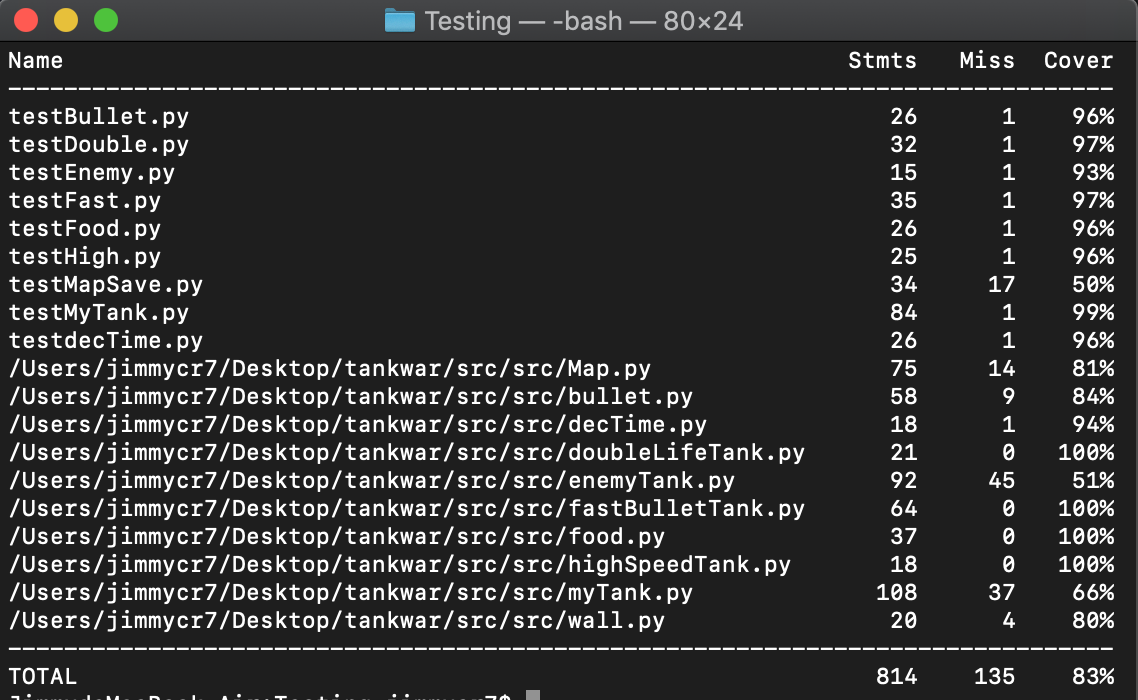
\includegraphics[scale=0.7]{coverage.png}
\caption{Coverage Test Screenshot}
\label{Coverage Test}
\end{figure}

\bibliographystyle{plainnat}

\bibliography{SRS}

\end{document}